\section{Results}
\label{sec:results}

We tested our model using the following metrics: epoch loss, pixel accuracy, IoU score, and dice score.

\begin{table}[htbp]
    \centering
    \caption{Training performance metrics}
    \label{tab:example}

    \begin{tabular}{|c|c|c|}
        \hline
        \textbf{} & \textbf{Background} & \textbf{Muscle layer} \\
        \hline
        \textbf{Pixel accuracy} & 0.8852 & 0.8852 \\
        \textbf{IoU score} & 0.8312 & 0.6159 \\
        \textbf{Dice score} & 0.4528 & 0.3423 \\
        \textbf{F1 score} & 0.9056 & 0.6846 \\
        \hline
    \end{tabular}

    \begin{tabular}{|c|c|c|}
        \hline
        \textbf{} & \textbf{Mucosal layer} & \textbf{Electrode} \\
        \hline
        \textbf{Pixel accuracy} & 0.8852 & 0.8852 \\
        \textbf{IoU score} & 0.2282 & 0.4474 \\
        \textbf{Dice score} & 0.1339 & 0.2656 \\
        \textbf{F1 score} & 0.2678 & 0.5312 \\
        \hline
    \end{tabular}

\end{table}

\begin{figure}[htp!]
    \centering
    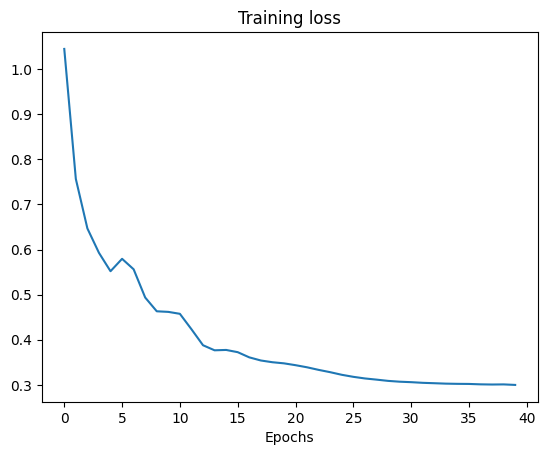
\includegraphics[width=0.4\textwidth]{Images/loss.png}
    \caption{Training loss}
    \label{fig:loss}
\end{figure}

\begin{figure}[htp!]
    \centering
    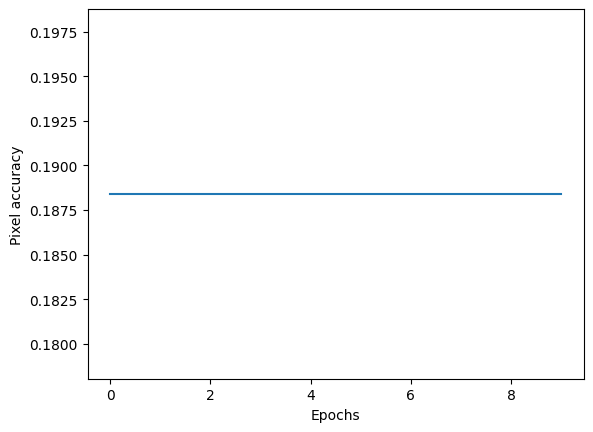
\includegraphics[width=0.4\textwidth]{Images/accuracy.png}
    \caption{Pixel accuracy}
    \label{fig:accuracy}
\end{figure}

\begin{figure}[htp!]
    \centering
    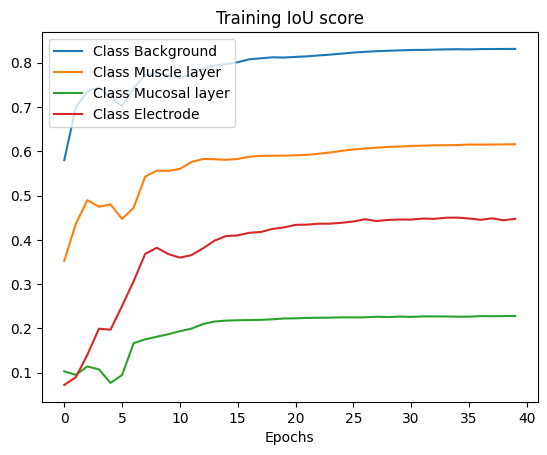
\includegraphics[width=0.4\textwidth]{Images/iou.png}
    \caption{IoU score}
    \label{fig:iou}
\end{figure}

\begin{figure}[htp!]
    \centering
    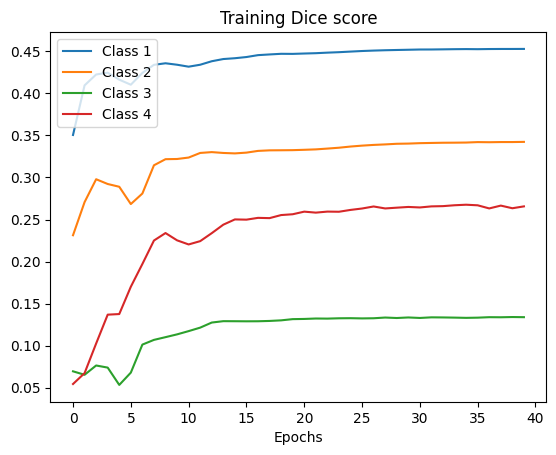
\includegraphics[width=0.4\textwidth]{Images/dice.png}
    \caption{Dice score}
    \label{fig:dice}
\end{figure}

\begin{figure}[htp!]
    \centering
    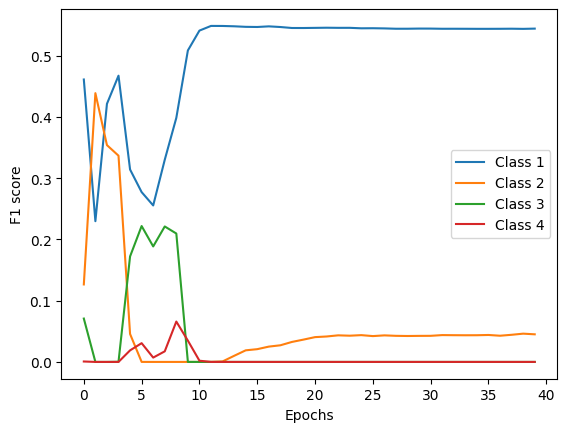
\includegraphics[width=0.4\textwidth]{Images/f1.png}
    \caption{F1 score}
    \label{fig:f1}
\end{figure}
